\usetikzlibrary{arrows}
%\usetikzlibrary{shapes.multipart}
\renewcommand{\arraystretch}{0.8}
\resizebox{\textwidth}{!}{
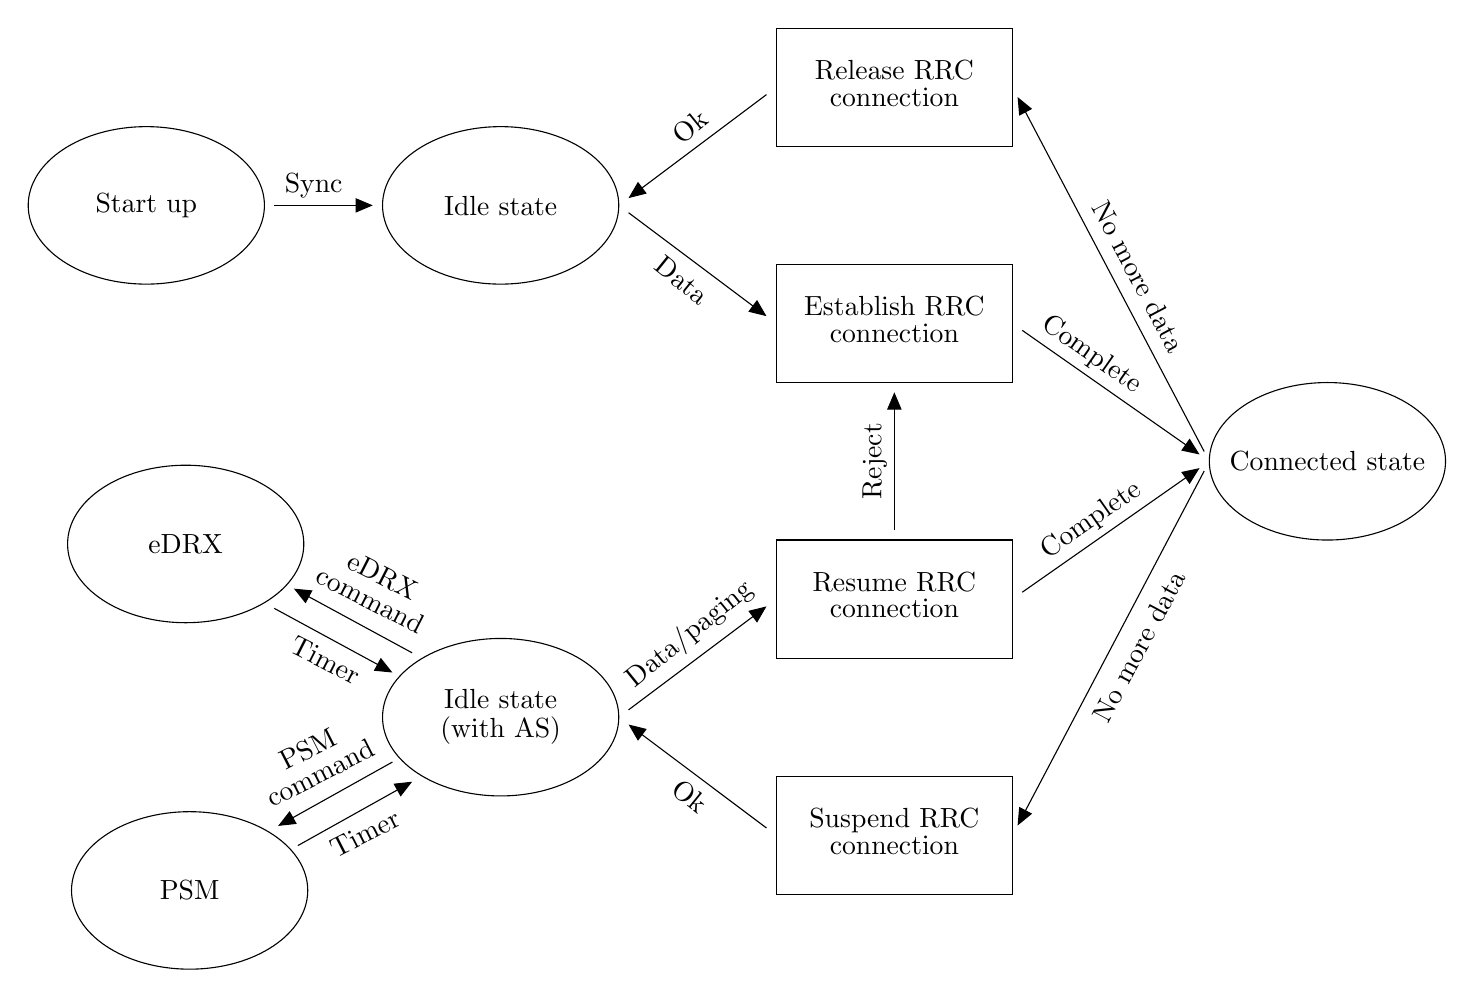
\begin{tikzpicture}[scale=0.5]

\draw  (-26,28) ellipse (3 and 2);
\node at (-26,28) {Start up};

\draw  (-17,28) ellipse (3 and 2);
\node at (-17,28) {Idle state};

\draw  (-24.9,10.6) ellipse (3 and 2);
%\node at (-17,15) {\acrshort{PSM}};
\node at (-24.9,10.6) {PSM};

\draw  (-10,19.5) rectangle (-4,16.5);
\node at (-7,18) {\begin{tabular}{c} Resume RRC \\ connection \end{tabular}};

\draw  (-10,26.5) rectangle (-4,23.5);
\node at (-7,25) {\begin{tabular}{c} Establish RRC \\ connection\end{tabular}};

\draw  (-10,13.5) rectangle (-4,10.5);
\node at (-7,12) {\begin{tabular}{c} Suspend RRC \\ connection\end{tabular}};

\draw  (-10,32.5) rectangle (-4,29.5);
\node at (-7,31) {\begin{tabular}{c} Release RRC \\ connection\end{tabular}};

\draw  (4,21.5) ellipse (3 and 2);
\node at (4,21.5) {Connected state};

\draw  (-17,15) ellipse (3 and 2);
\node at (-17,15) {\begin{tabular}{c} Idle state \\ (with AS)\end{tabular}};
\node (v22) at (-20,15) {};
\node (v23) at (-14,15) {};

\draw  (-25,19.4) ellipse (3 and 2);
\node at (-25,19.4) {eDRX};
\node (v25) at (-19,16.5) {};
\node (v26) at (-22.5,18.4) {};
\node (v27) at (-23,17.9) {};
\node (v28) at (-19.5,16) {};
\node[rotate=27] at (-21.7,13.8) {\begin{tabular}{c} PSM\\ command\end{tabular}};
\node[rotate=27] at (-20.45,12.05) {Timer};




\node (v1) at (-23,28) {};
\node (v2) at (-20,28) {};
\node (v3) at (-14,28) {};
\node (v4) at (-10,25) {};
\node (v5) at (-4,25) {};
\node (v6) at (1,21.5) {};
\node (v7) at (-4,12) {};
\node (v8) at (-4,31) {};
\node (v9) at (-4,18) {};
\node (v10) at (-10,18) {};
\node (v11) at (-10,12) {};
\node (v12) at (-10,31) {};
\node (v13) at (-7,19.5) {};
\node (v14) at (-7,23.5) {};
\node (v15) at (-19.5,14) {};
\node (v16) at (-22.9,12.1) {};
\node (v17) at (-22.4,11.6) {};
\node (v18) at (-19,13.5) {};



\draw [arrows={- triangle 45}] (v1) edge (v2);
\draw [arrows={- triangle 45}] (v23) edge (v10);
\draw [arrows={- triangle 45}] (v3) edge (v4);
%\draw [arrows={triangle 45-}]  (v4) edge ($(midpoint)+(0,0)$);

\draw [arrows={- triangle 45}] (v11) edge (v23);
\draw [arrows={- triangle 45}] (v12) edge (v3);
\draw [arrows={- triangle 45}] (v13) edge (v14);
\draw [arrows={- triangle 45}] (v9) edge (v6);
\draw [arrows={- triangle 45}] (v5) edge (v6);
\draw [arrows={- triangle 45}] (v6) edge (v7);
\draw [arrows={- triangle 45}] (v6) edge (v8);
\draw [arrows={- triangle 45}] (v15) edge (v16);
\draw [arrows={- triangle 45}]  (v17) edge (v18);
\draw [arrows={- triangle 45}] (v25) edge (v26);
\draw [arrows={- triangle 45}]  (v27) edge (v28);


\node at (-21.75,28.5) {Sync};
\node[rotate=-27] at (-20.2,18.2) {\begin{tabular}{c} eDRX \\ command\end{tabular}};
\node[rotate=-27] at (-21.45,16.45) {Timer};
\node[rotate=39] at (-12.2,30) {Ok};
\node[rotate=39] at (-12.2,17.1) {Data/paging};
\node[rotate=-39] at (-12.2,13) {Ok};
\node[rotate=-39] at (-12.4,26.1) {Data};
\node[rotate=-35] at (-2,24.2) {Complete};
\node[rotate=35] at (-2,20) {Complete};
\node[rotate=62] at (-0.8,16.8) {No more data};
\node[rotate=-62] at (-0.8,26.2) {No more data};
\node[rotate=90] at (-7.5,21.5) {Reject};


\end{tikzpicture}
}